\subsection{PLA (Programmable Logic Array)}
Programmable Logic Array (PLA) es un dispositivo lógico de arquitectura fija con puertas AND programables seguidas de puertas OR programables. PLA es básicamente un tipo de dispositivo lógico programable que se utiliza para construir un circuito digital reconfigurable. La estructura de un PLA es la siguiente:

\begin{figure}[h]
    \centering
    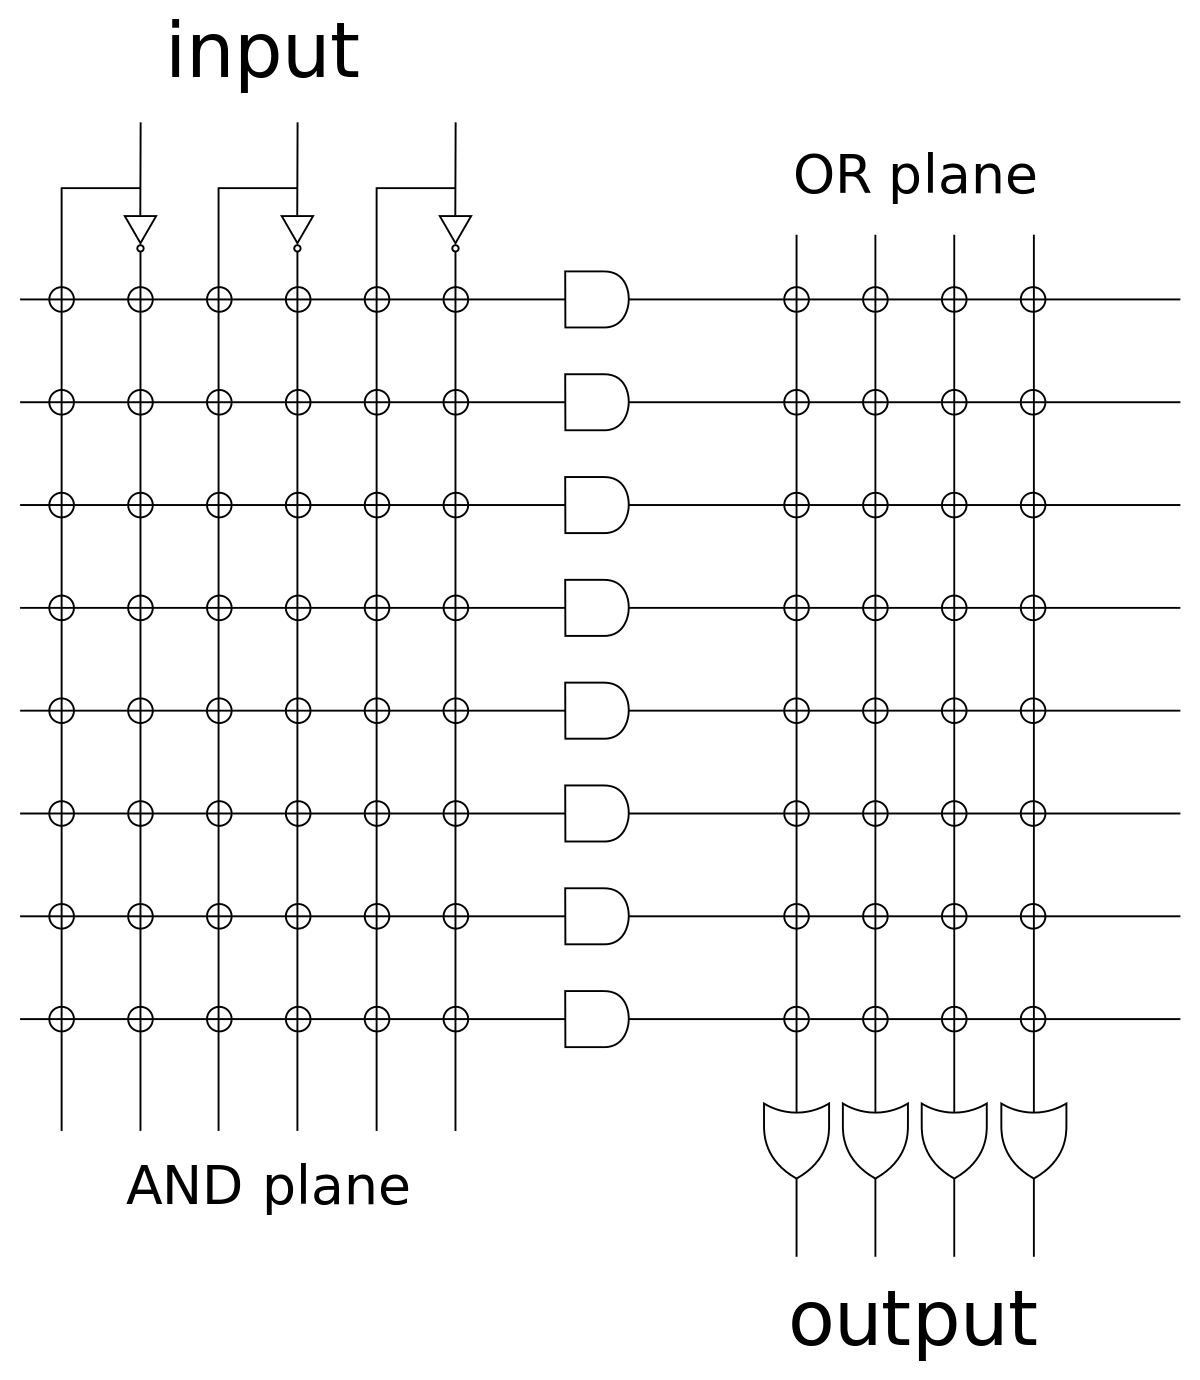
\includegraphics[scale=0.2]{img/pla.png}
    \caption{Estructura de un PLA}
\end{figure}

El funcionamiento se podria resumir en tres pasos:

\begin{enumerate}
    \item \textbf{Programación:} el usuario define la función lógica que se desea implementar.
    \item \textbf{Generación de términos del producto:} las entradas se aplican a la matriz de puertas AND para producir un conjunto de términos de producto.
    \item \textbf{Generación de suma de términos:} los términos de producto se aplican a la matriz de puertas OR para producir la salida.
\end{enumerate}

\newpage
\subsubsection{Método para implementar una función lógica en un PLA}
\begin{mdframed}[backgroundcolor=gray!10,linewidth=0]
    \begin{enumerate}
        \item Una vez se tenga la función lógica simplificada, se deben identificar los términos de la función.
        \item Cada término de la función se convierte en una fila de la matriz de puertas AND.
        \item Luego se suman los términos de la función y se convierten en una fila de la matriz de puertas OR.
        \item La salida de la matriz de puertas OR es la función lógica implementada en el PLA.
    \end{enumerate}
\end{mdframed}
